% ============================================
% SECTION 4: METHODOLOGICAL FRAMEWORK
% How We Measure Cognitive Sovereignty
% ============================================
%
% REVISION v2 NOTES:
% Incorporated all nine repairs from external review:
% 1. Equation consistency (S = P_brain × α_synth × R)
% 2. Removed "pre-emptive insult" circularity defense
% 3. Fixed Efficiency Inversion table (dropped cost column)
% 4. Clarified geometry as metaphor, properties as observable
% 5. Flagged medieval/modern as "Illustrative scenario"
% 6. Made Cynefin mapping ordinal (not numeric constants)
% 7. Reframed Kolmogorov as approximate compressibility
% 8. Added placeholder note for decay λ values
% 9. Renamed veterinary section to "Comparative Case Illustration"
% ============================================

\section{Methodological Framework: Measuring Cognitive Sovereignty}
\label{sec:methodology}

This section presents the analytical tools for measuring cognitive sovereignty: the core equation grounded in neurological constraints, the R-value framework for quantifying extraction resistance, and validation through contemporary evidence.

\subsection{The Power-Budget Allocation Model}

Cognitive sovereignty can be expressed as a power-budget allocation:

\begin{equation}
S = P_{brain} \times \alpha_{synth} \times R
\label{eq:sovereignty}
\end{equation}

\noindent Where:
\begin{itemize}
    \item $P_{brain} \approx 20$W represents baseline cerebral metabolism—the remarkably constant power consumption of the human brain \citep{raichle2002}
    \item $\alpha_{synth} \in [0,1]$ represents the fraction of waking time allocated to synthesis-supporting cognitive states
    \item $R \in [0,1]$ represents extraction resistance—the architectural quality that determines vulnerability to algorithmic replication
\end{itemize}

This formulation grounds cognitive sovereignty in the same energetic analysis that \citet{smil2017} employs to trace civilizational transitions. Just as Smil demonstrates that societal complexity requires specific power densities, cognitive complexity requires specific allocations of the brain's fixed power budget. The model doesn't pretend to measure Joules directly; it allocates a known baseline according to observable time-use patterns.

The key constraint: Energy Investment Rate must exceed Entropy Rate. Without sustained allocation toward synthesis, cognitive architecture degrades toward maximum entropy—the thermodynamic floor where patterns become simple enough for extraction.

\subsection{Clarifying the Energy Constraint}
\label{sec:energy-constraint}

We treat energy as a constraint grounded in neuroscience, not mere metaphor. The human brain consumes approximately 20 Watts continuously—roughly 20\% of the body's resting metabolism despite comprising only 2\% of body mass \citep{raichle2002}. This baseline is remarkably constant. Task-evoked increases for ``hard thinking'' add surprisingly little whole-brain energy: recent reviews estimate only 5\% above baseline for goal-directed cognition \citep{jamadar2025}. A student cramming for examinations and a scholar staring contemplatively at clouds consume nearly identical metabolic power.

The meaningful variable, therefore, is not \textit{total} energy expenditure but the \textit{allocation} of this constant baseline across cognitive states. Neuroscience distinguishes between task-positive states (goal-directed, externally focused, deploying existing cognitive structures) and default-mode network (DMN) states that support consolidation, recombination, and creative incubation \citep{raichle2001}. The DMN activates during mind-wandering, autobiographical integration, semantic association, and simulation of futures—precisely the mental terrain where ``shower insights'' emerge and cross-domain synthesis occurs.

The synthesis allocation fraction ($\alpha_{synth}$) captures this: what proportion of the brain's constant 20W flows toward DMN-dominant integration versus task-positive execution?

\textit{Illustrative scenario}: Consider two schematic cognitive regimes, acknowledging that historical and contemporary time-use varies widely across contexts:

\textbf{The Medieval Scholar}:
\begin{itemize}
    \item 4 hours formal study and lectures (task-positive)
    \item 4 hours disputation, pub debate, contemplative walking (DMN synthesis)
    \item Survival needs largely externalized (institutional support)
    \item Synthesis allocation: $\alpha_{synth} \approx 0.25$
    \item Effective synthesis power: $20\text{W} \times 0.25 = \mathbf{5\text{W}}$
\end{itemize}

\textbf{The Modern Knowledge Worker}:
\begin{itemize}
    \item 8--10 hours employment (task-positive, vector execution)
    \item 2 hours commuting (stress and vigilance, not synthesis)
    \item 2 hours domestic labor and administrative survival
    \item 2 hours passive screen recovery
    \item Synthesis allocation: $\alpha_{synth} \approx 0.03$
    \item Effective synthesis power: $20\text{W} \times 0.03 = \mathbf{0.6\text{W}}$
\end{itemize}

In this illustrative scenario, the ratio could be on the order of 5--10$\times$. The precise magnitude awaits rigorous historical time-use analysis; the directional claim—that synthesis allocation has collapsed dramatically—is robust across plausible parameterizations. The pub wasn't leisure; it was \textit{infrastructure for cognitive integration}. The wandering between monasteries wasn't inefficiency; it was \textit{incubation time}. What we now optimize away as waste may have been producing much of the value.

\subsection{The Efficiency Inversion Paradox}

Here the thermodynamic analysis becomes most striking.

Medieval civilization paid \textit{enormously} for each hour of scholarly capacity. With 90\% of the population required for food production, supporting a single scholar-year consumed substantial agricultural surplus. Shelter, heating, manuscript production, institutional overhead—the civilizational cost per unit of protected cognitive time was staggering by modern standards.

Yet they \textit{allocated} that hard-won cognitive time generously to synthesis. Disputations. Contemplation. The informal collisions of pub and plaza. Students were permitted—expected—to integrate without immediate productive output.

Modern civilization pays \textit{trivially} for cognitive capacity. Food production requires 2\% of the population. Shelter, heating, and information access are historically cheap. The civilizational cost per student-year has collapsed by orders of magnitude.

Yet we \textit{capture} that cheap cognitive time entirely for vectorized production. No disputation time—replaced by measurable learning outcomes. No wandering—replaced by optimized credit accumulation. No protected integration—every hour scheduled, productive, accountable.

\begin{table}[htbp]
\centering
\begin{tabular}{lcc}
\toprule
\textbf{Era} & \textbf{Synthesis Allocation ($\alpha_{synth}$)} & \textbf{Effective Synthesis Power} \\
\midrule
Medieval (illustrative) & $\sim$25\% & $\sim$5W \\
Modern (illustrative) & $\sim$3\% & $\sim$0.6W \\
\midrule
\textbf{Ratio} & \multicolumn{2}{c}{$\sim$5--10$\times$ reduction} \\
\bottomrule
\end{tabular}
\caption{The Efficiency Inversion (illustrative estimates). Despite commanding vastly greater resources, modern systems allocate dramatically less cognitive power toward synthesis. We optimized away the apparent ``waste'' that was generating integrative capacity. Precise historical values require dedicated time-use research; the directional collapse is robust.}
\label{tab:efficiency-inversion}
\end{table}

The pattern is consistent: resource-poor medieval civilization protected synthesis allocation; resource-rich modern civilization eliminates it. The 88\% transformation failure rate, the 42\% AI project abandonment, the German engineers restoring the Diplom they sacrificed to Bologna: these may be returns on our efficiency optimization—vectors optimized, spheres starved.

\subsection{Falsifiable Predictions}

The claim that ``protected synthesis time grows cognitive architecture'' while ``task-positive execution deploys existing architecture'' generates testable predictions:

\begin{enumerate}
    \item \textbf{Network Prediction}: Broad learning combined with protected idle time should increase cross-network coupling (DMN$\leftrightarrow$frontoparietal control networks) and produce richer resting-state connectivity patterns, measurable via functional neuroimaging. Intensive vector training without integration time should show reduced cross-network coupling.
    
    \item \textbf{Behavioral Prediction}: Individuals with protected synthesis time should demonstrate superior far transfer, analogical reasoning, and insight problem-solving after incubation periods, compared to equivalent total hours spent on concentrated specialization without integration time.
    
    \item \textbf{Structural Prediction}: Concept maps and semantic networks elicited from broad-study participants should show higher ``bridging'' coefficients (connections between distant conceptual clusters) and greater redundancy (multiple paths between nodes), compared to specialists with equivalent total study time.
    
    \item \textbf{Institutional Prediction}: Educational programs preserving protected synthesis time (traditional liberal arts curricula, the German Diplom model, apprenticeship structures) should produce graduates with measurably higher performance on complex-domain tasks and lower susceptibility to AI substitution, controlling for total instructional hours.
\end{enumerate}

These predictions operationalize sphere-building through observable differences in networks, behaviors, structures, and institutional outcomes. The framework invites empirical validation rather than requiring acceptance on theoretical grounds alone.

\subsection{The R-Value Framework}

The second component of cognitive sovereignty—Resistance to Extraction ($R$)—quantifies architectural quality. We propose R as an operational definition: cognitive quality \textit{manifests as} resistance to algorithmic extraction. High-quality architecture exhibits properties (cross-domain connectivity, contextual adaptability, emergent synthesis) that current extraction methods cannot capture. Low-quality architecture exhibits properties (linear procedures, standardized outputs, context-independence) that map directly to algorithmic implementation.

This is operational definition, not circular reasoning. R earns legitimacy through predictive and explanatory performance: does framing cognitive architecture in terms of extraction resistance successfully illuminate transformation failure rates, AI substitution patterns, and institutional outcomes? The falsifiable predictions above provide the validation pathway. We invite skeptical engagement with these specific empirical claims.

Table~\ref{tab:r-values} presents the R-value framework with corresponding geometric, domain, and technological correlates:

\begin{table}[htbp]
\centering
\begin{tabular}{lllll}
\toprule
\textbf{R Range} & \textbf{Geometry} & \textbf{Cynefin Domain} & \textbf{Exemplar} & \textbf{AI Status} \\
\midrule
High (0.7--0.9) & Sphere & Chaotic & Renaissance polymath & Beyond current horizon \\
Moderate-High (0.4--0.7) & Ellipsoid & Complex & Complex navigator & Theoretical ceiling \\
Moderate (0.2--0.4) & Cylinder & Complicated & Domain specialist & Current frontier \\
Low (0.0--0.2) & Vector & Clear & Procedural executor & Substantially automated \\
\bottomrule
\end{tabular}
\caption{R-value framework mapping extraction resistance to cognitive geometry, Cynefin domains, and AI capability boundaries. Ranges represent theoretical positions based on documented characteristics; boundaries require empirical validation through the predictions specified in Section~\ref{sec:energy-constraint}.}
\label{tab:r-values}
\end{table}

These are theoretical positions enabling comparative analysis, not validated measurements. We \textit{define} a Renaissance polymath as exhibiting high R based on demonstrated capacity for cross-domain synthesis that resisted standardization for centuries. We \textit{position} current LLMs at low R based on observable performance differentials between procedural and emergent domains. The framework's value lies in its explanatory coherence across documented phenomena rather than predictive precision—precision that future empirical work can provide.

\subsection{Measurement Approaches for R}

We propose multiple measurement approaches, recognizing that R manifests differently across contexts:

\begin{enumerate}
    \item \textbf{Dimensional Diversity ($R_1$)}: $R = 1 - (1/n)$, where $n$ represents meaningfully integrated knowledge domains—not mere exposure but demonstrated synthesis capacity. This provides a lower bound; integration quality matters beyond domain count.
    
    \item \textbf{Network Density ($R_2$)}: Ratio of actual to possible conceptual connections in elicited knowledge structures, measurable through concept mapping methodologies \citep{novak1984}.
    
    \item \textbf{Approximate Compressibility ($R_3$)}: The degree to which cognitive output resists compression—operationalized through compression ratios on written explanations, minimum description length of concept representations, or model-based predictability metrics. High-R outputs require longer descriptions; low-R outputs compress efficiently.
    
    \item \textbf{Cynefin Classification ($R_4$)}: Domain-specific resistance based on task complexity—Clear domains afford low R, Complicated domains moderate R, Complex domains high R, Chaotic domains very high R. These ordinal rankings reflect documented performance differentials across domain types; precise numeric mapping awaits empirical validation.
    
    \item \textbf{Transfer Performance ($R_5$)}: Demonstrated capability on novel problems outside training distribution—the behavioral signature of sphere architecture, measurable through far-transfer tasks and cross-domain application assessments.
\end{enumerate}

Practitioners may employ individual metrics or weighted combinations ($R = \sum w_i \times R_i$) appropriate to their specific assessment context. The plurality of approaches reflects the multidimensional nature of cognitive architecture—no single index captures it fully, but multiple indices can triangulate the underlying structure.

\subsection{Temporal Dynamics: Decay Without Maintenance}

Resistance exhibits temporal decay without sustained investment:

\begin{equation}
R(t) = R_0 \times e^{-\lambda t}
\label{eq:decay}
\end{equation}

\noindent where $\lambda$ represents domain-specific decay rates. We propose illustrative ranges based on documented forgetting patterns and skill degradation literature \citep{murre2015}: from approximately 0.05/year for deeply embodied skills with regular but infrequent use, to approximately 1.0/year for shallow credentials without reinforcement. These are placeholder parameters requiring empirical fitting; the functional form captures the thermodynamic reality that cognitive architecture degrades without energy investment. Skills unused decay; credentials unexercised become meaningless; the Second Law operates on knowledge as on all organized complexity.

\subsection{Sphere Versus Vector: Architectural Properties}

The geometric language—sphere, vector, cylinder, ellipsoid—is compact metaphor for observable network and behavioral properties. What we call ``sphere architecture'' manifests as measurable characteristics; the metaphor earns its keep through predictive utility, not literal correspondence.

\textbf{Sphere Architecture} (high R) manifests as:
\begin{itemize}
    \item Dense cross-domain connections enabling novel synthesis (measurable via concept mapping)
    \item Multiple paths between concepts—network redundancy (measurable via graph analysis)
    \item Adaptive capacity across unfamiliar contexts (measurable via transfer tasks)
    \item Emergent insight from dimensional interaction (measurable via creative problem-solving)
    \item Built through sustained DMN-dominant synthesis allocation
    \item Resistance to extraction through irreducible complexity
\end{itemize}

\textbf{Vector Architecture} (low R) manifests as:
\begin{itemize}
    \item Linear specialization along predetermined pathways (measurable via knowledge structure elicitation)
    \item Minimal cross-connections between knowledge domains (measurable via bridging coefficients)
    \item Efficiency within bounded, familiar contexts (measurable via routine task performance)
    \item Procedural responses to categorized inputs (measurable via protocol adherence)
    \item Built through task-positive training without integration time
    \item Vulnerability to extraction through complete documentability
\end{itemize}

The sphere-to-vector transformation appears in observable changes: declining breadth of study, increasing specialization, elimination of protected integration time, reduced cross-domain practice. These are measurable educational and institutional patterns, not just theoretical constructs.

\subsection{The Foundation-Specialization Ratio}

Historical analysis reveals a critical architectural metric: the proportion of educational investment devoted to comprehensive foundations versus specialized applications. Figure~\ref{fig:foundation-specialization} traces this ratio across 2,500 years.

\begin{figure}[htbp]
    \centering
    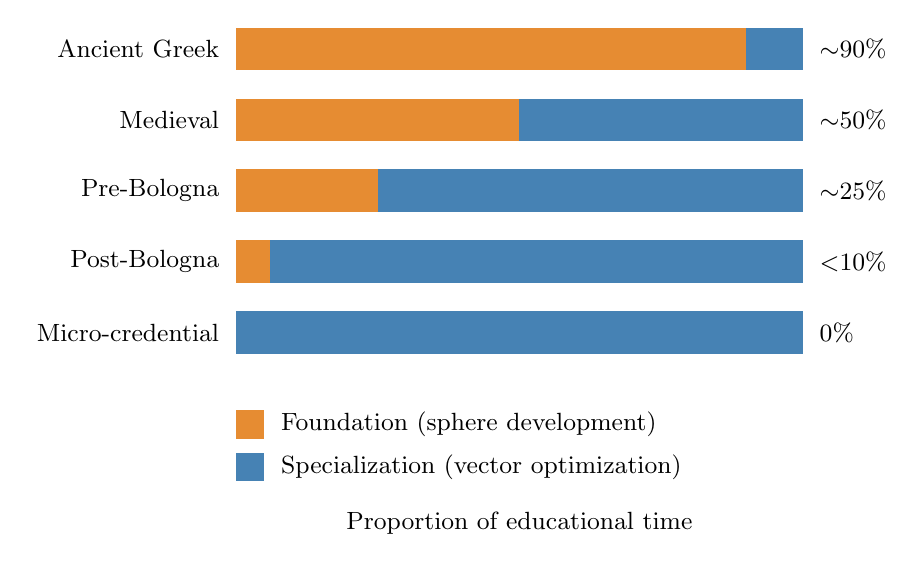
\begin{tikzpicture}[scale=0.9]
        % Define bar properties
        \def\barheight{0.6}
        \def\barwidth{8}
        \def\spacing{1.0}
        
        % Foundation color (orange/warm) and Specialization color (cold blue)
        \definecolor{foundation}{RGB}{230, 140, 50}
        \definecolor{specialization}{RGB}{70, 130, 180}
        
        % Ancient Greek: 90% foundation
        \fill[foundation] (0, 5*\spacing) rectangle (0.90*\barwidth, 5*\spacing+\barheight);
        \fill[specialization] (0.90*\barwidth, 5*\spacing) rectangle (\barwidth, 5*\spacing+\barheight);
        \node[left] at (-0.1, 5*\spacing+\barheight/2) {\small Ancient Greek};
        \node[right] at (\barwidth+0.1, 5*\spacing+\barheight/2) {\small $\sim$90\%};
        
        % Medieval: 50% foundation
        \fill[foundation] (0, 4*\spacing) rectangle (0.50*\barwidth, 4*\spacing+\barheight);
        \fill[specialization] (0.50*\barwidth, 4*\spacing) rectangle (\barwidth, 4*\spacing+\barheight);
        \node[left] at (-0.1, 4*\spacing+\barheight/2) {\small Medieval};
        \node[right] at (\barwidth+0.1, 4*\spacing+\barheight/2) {\small $\sim$50\%};
        
        % Pre-Bologna: 25% foundation
        \fill[foundation] (0, 3*\spacing) rectangle (0.25*\barwidth, 3*\spacing+\barheight);
        \fill[specialization] (0.25*\barwidth, 3*\spacing) rectangle (\barwidth, 3*\spacing+\barheight);
        \node[left] at (-0.1, 3*\spacing+\barheight/2) {\small Pre-Bologna};
        \node[right] at (\barwidth+0.1, 3*\spacing+\barheight/2) {\small $\sim$25\%};
        
        % Post-Bologna: <10% foundation
        \fill[foundation] (0, 2*\spacing) rectangle (0.06*\barwidth, 2*\spacing+\barheight);
        \fill[specialization] (0.06*\barwidth, 2*\spacing) rectangle (\barwidth, 2*\spacing+\barheight);
        \node[left] at (-0.1, 2*\spacing+\barheight/2) {\small Post-Bologna};
        \node[right] at (\barwidth+0.1, 2*\spacing+\barheight/2) {\small $<$10\%};
        
        % Micro-credential: 0% foundation
        \fill[specialization] (0, 1*\spacing) rectangle (\barwidth, 1*\spacing+\barheight);
        \node[left] at (-0.1, 1*\spacing+\barheight/2) {\small Micro-credential};
        \node[right] at (\barwidth+0.1, 1*\spacing+\barheight/2) {\small 0\%};
        
        % Legend - stacked vertically, left-aligned
        \fill[foundation] (0, -0.2) rectangle (0.4, 0.2);
        \node[right] at (0.5, 0) {\small Foundation (sphere development)};
        
        \fill[specialization] (0, -0.8) rectangle (0.4, -0.4);
        \node[right] at (0.5, -0.6) {\small Specialization (vector optimization)};
        
        % X-axis label
        \node at (4, -1.4) {\small Proportion of educational time};
    \end{tikzpicture}
    \caption{\textbf{The Foundation-Specialization Inversion (500 BCE--2025 CE).} Historical educational systems invested heavily in comprehensive foundations before permitting specialization. The architectural inversion correlates with declining extraction resistance. Percentages are approximate, derived from documented curriculum structures; the inversion pattern is robust across sources.}
    \label{fig:foundation-specialization}
\end{figure}

The pattern reveals two simultaneous collapses:

\begin{enumerate}
    \item \textbf{Total duration reduction}: From 20+ years of sustained development to 40-hour micro-credentials—orders of magnitude decrease in total investment
    \item \textbf{Foundation elimination}: From $\sim$90\% sphere-building to effectively 0\%—complete architectural inversion
\end{enumerate}

The combination illuminates why modern credentials may produce specialists vulnerable to AI replacement: narrow vectors built on minimal spherical foundations, with no protected synthesis time during which the constant 20W baseline might have grown integrative architecture.

\subsection{Comparative Case Illustration: Veterinary Medicine}

The framework gains illustrative support through contemporary comparison of educational structures producing different extraction resistance despite similar duration.

Human medicine and veterinary medicine both require approximately 8 years of post-secondary education. Yet their cognitive architectures appear to differ:

\textbf{Human Medicine (Specialist Tendency)}:
\begin{itemize}
    \item Early specialization into organ systems and subspecialties
    \item Protocol-driven diagnostic pathways
    \item Single-species optimization
    \item Increasing reliance on algorithmic decision support
\end{itemize}

\textbf{Veterinary Medicine (Generalist Tendency)}:
\begin{itemize}
    \item Comprehensive foundation across multiple species
    \item Pattern-recognition across biological diversity
    \item Continuous context-switching between anatomies
    \item Adaptive reasoning without species-specific protocols for many conditions
\end{itemize}

\citet{lewis2022} document a ``scanning approach'' characteristic of veterinary clinical reasoning: broad initial assessment followed by contextual narrowing, contrasting with linear algorithm application. \citet{vandeweerd2013} note that veterinary expertise requires integration across ``widely different species and conditions.''

This comparison suggests a testable hypothesis rather than established proof: \textbf{same duration, different architecture, potentially different R-values}. Time investment alone may not determine extraction resistance; architectural choices during that investment—whether the constant 20W flows toward cross-domain synthesis or toward single-domain optimization—may determine whether the result trends toward sphere or vector. Rigorous comparative study could validate or refute this hypothesis.

As veterinarians sometimes note: ``Real doctors treat more than one species.'' The quip may contain architectural truth worth empirical investigation.

\subsection{Methodological Limitations and Scope}

This framework operates at the level of structural analysis rather than individual prediction. We identify architectural patterns that correlate with extraction resistance without claiming to measure any individual's precise R-value. The equation provides diagnostic and comparative tools, not personality assessment.

Several limitations require acknowledgment:

\begin{itemize}
    \item \textbf{R-values are theoretical positions} requiring validation through the specified predictions. We do not claim to have measured spheres; we claim to have specified how they could be measured.
    
    \item \textbf{Historical estimates are illustrative}. The medieval/modern comparison uses schematic values; precise historical synthesis-allocation data requires dedicated research beyond this paper's scope.
    
    \item \textbf{Decay parameters ($\lambda$) are placeholders} derived from general forgetting-curve patterns, not fitted to cognitive-architecture-specific data.
    
    \item \textbf{The veterinary comparison is hypothesis-generating}, not hypothesis-confirming. It suggests a natural experiment; it doesn't complete one.
\end{itemize}

What the framework \textit{does} establish is the thermodynamic constraint: cognitive architectures require sustained allocation of the brain's constant baseline power toward synthesis states, and extraction resistance correlates with that allocation over time. This is a physical relationship grounded in neuroscience—baseline metabolism, DMN function, network coupling—not preference dressed as physics.

The framework generates specific, testable predictions. Its ultimate value depends on whether those predictions survive empirical scrutiny. We offer it as a lens that illuminates documented phenomena—transformation failures, AI substitution patterns, institutional resistance—while inviting the validation that would transform illumination into explanation.

Section~\ref{sec:historical} examines why historical systems succeeded in protecting synthesis allocation while contemporary systems systematically eliminate it.

% ============================================
% END SECTION 4
% ============================================
%
% CITATIONS USED:
% - Smil (2017) - energy transitions
% - Raichle & Gusnard (2002) - brain baseline metabolism  
% - Raichle et al. (2001) - default mode network
% - Jamadar (2025) - metabolic costs of cognition
% - Lewis et al. (2022) - veterinary clinical reasoning
% - Vandeweerd et al. (2012) - veterinary expertise
% - Novak & Gowin (1984) - concept mapping [ADD TO BIB]
% - Murre & Dros (2015) - forgetting curves [ADD TO BIB]
%
% NEW CITATIONS TO ADD TO references.bib:
%
% @article{raichle2001,
%   author = {Raichle, Marcus E. and MacLeod, Ann Mary and Snyder, Abraham Z. 
%             and Powers, William J. and Gusnard, Debra A. and Shulman, Gordon L.},
%   title = {A default mode of brain function},
%   journal = {Proceedings of the National Academy of Sciences},
%   volume = {98},
%   number = {2},
%   pages = {676--682},
%   year = {2001}
% }
%
% @book{novak1984,
%   author = {Novak, Joseph D. and Gowin, D. Bob},
%   title = {Learning How to Learn},
%   publisher = {Cambridge University Press},
%   year = {1984}
% }
%
% @article{murre2015,
%   author = {Murre, Jaap M. J. and Dros, Joeri},
%   title = {Replication and Analysis of Ebbinghaus' Forgetting Curve},
%   journal = {PLOS ONE},
%   volume = {10},
%   number = {7},
%   pages = {e0120644},
%   year = {2015}
% }
%
% ============================================
% REPAIRS INCORPORATED (v2):
% 1. ✓ Equation now S = P_brain × α_synth × R (allocation model)
% 2. ✓ Removed hostile circularity defense language
% 3. ✓ Efficiency table simplified (dropped cost column)
% 4. ✓ "Geometric language is compact metaphor for observable properties"
% 5. ✓ Medieval/modern flagged as "Illustrative scenario"
% 6. ✓ Cynefin mapping now ordinal (Low/Moderate/High/Very High)
% 7. ✓ Kolmogorov reframed as "Approximate Compressibility"
% 8. ✓ Decay λ explicitly noted as "placeholder parameters"
% 9. ✓ Veterinary renamed "Comparative Case Illustration"
% ============================================